\section{Feil og feilanalyse: FMECA}
\label{sec:fmeca}


\subsection{FMECA intro}

FMECA står for FeilMode Effekt (C)Konsekvens/kritikalitet Analyse og er en metodikk for å analysere feilmoder. Det er en systematisk og strukturert metode med fast oppsett, hvor resultatet presenteres i en FMECA-tabell, se eksempel i figur \ref{fig:fmeca_propell}.

\begin{figure}[H]
    \centering
        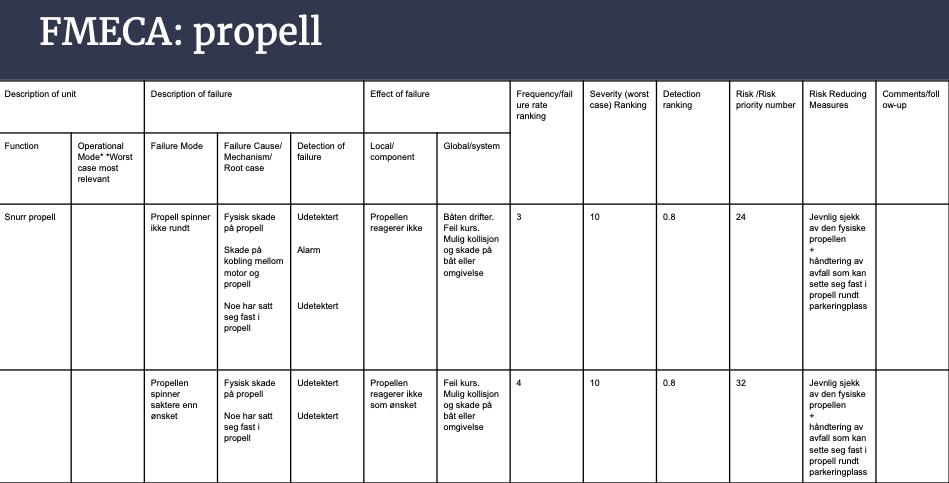
\includegraphics[width=\textwidth]{figures/FMECA/Skjermbilde 2021-11-24 kl. 09.54.55.png}\\
        \caption{Eksempel på FMECA-tabell for propell på båt.}
        \label{fig:fmeca_propell}
\end{figure}

FMECA brukes til å identifisere alle potensielle feilmoder av forskjellige deler av et system, konsekvensene av disse feilmodene, og hvordan vi kan unngå eller minske effekten av feilene.

FMECA er en teknikk for å identifisere, prioritere og eliminere potensielle feil fra et system, design eller prosess før de når kunden.


Ved hjelp av FMECA kan vi få et anslag av systemets \textbf{diagnostic coverage}, det vil si, hvor effektiv vi oppfatter feil i systemet. Matematisk er dette en ratio gitt av forholdet mellom antall detekterte feil, over totalt antall mulige feil.


\subsection{Bakgrunn}
\begin{itemize}
    \item FMECA er en av de tidligste formene for feilanalyse, og ble utviklet av det amerikanske militære.
    \item FMECA blir mest brukt i reliabilitetsanalyse i tidlig stadie i produkt/system-utvikling, vanligvis under konsept- og tidlig design-fase for å sikre at alle potensielle feilmoder har blitt evaluert og at man har på plass riktige tiltak for å eliminere disse feilene.
\end{itemize}

\subsection{Metode}

\textbf{I forkant av FMECA-prosedyren}

\begin{itemize}
    \item[\textbf{1:}] Definer systemet som skal analyseres.
    \begin{itemize}
        \item Systemgrenser (hva skal inkluderes og ikke)
        \item Systemets hovedoppgave og funksjon, inkludert funksjonskrav
        \item Operasjonelle og miljømessige tilstander som bør vurderes
    \end{itemize}
    \item[\textbf{2:}] Samle tilgjengelig informasjon som beskriver systemet som skal analyseres, feks. tegninger, spesifikajsoner, skjemaer ...
    \item[\textbf{3:}] Samle informasjon om tidligere og liknende design fra interne kilder, som intervjuer med designere, vedlikeholdspersonell, osv.
\end{itemize}

\textbf{FMECA-prosedyren}

\begin{itemize}
    \item[\textbf{1:}] Systemdekomponering: Del opp systemet i komponenter, gjerne funksjonelle elementer. Se eksempel i figur \ref{fig:decomp}. Systemdekomponering bør alltid gjennomføres på et høyt nivå, for så å gå i detaljer der hvor uakseptable konsekvenser finnes. 
    \item[\textbf{2:}] FMECA tabell: Hver komponent fra systemdekomponeringen skal analyseres. Alle funksjoner komponenten utøver skal inkluderes, fra alle operasjonsmodene. Deretter spør vi om komponentens feil kan føre til uakseptabel effekt på systemet. Hvis svaret er ja, må komponenten undersøkes videre. I en FMECA-tabell har vi følgende kolonner:
    \begin{itemize}
        \item \textbf{Unik referanse til element}: Eks ID eller tag nummer.
        \item \textbf{Funksjon}: Komponentens funksjoner listes opp. Viktig å liste alle funksjoner. 
        \item \textbf{Operasjonsmoder}: De forskjellige operasjonsmodene for komponenten listes. Eks: Idle, standby, running. Kan utelukkes om operasjonsmoder ikke er relevant.
        \item \textbf{Potensielle feilmoder}: Identifiser alle potensielle feilmoder for hver funksjon og operasjonsmode. En feilmode bør være en form av ikke-suksess for funksjonen. 
        \item \textbf{Årsaker}: Potensielle årsaker til alle potensielle feilmoder listes, eks korrosjon, slitasje.
        IEC61508 skiller på feilårsaker:
        \begin{itemize}
            \item Tilfeildige feil: Feil som kommer tilbake. Eks. Random hardware feil, slitasje, korrosjon. For å handles med tilfeldige feil må man introdusere feilrater og regelmessig testing.
            \item Systematiske feil: Feil som er deterministiske, f. eks. programmeringsfeil. DIsse feilene kan i utgangspunktet korrigeres 100\%. 
        \end{itemize}
        \item \textbf{Deteksjon}: Muligheten for deteksjon av de identifiserte feilmodene listes. Eks diagnostisk testing, menneskelig oppfatning. Noen feilmoder kan detekteres, andre kan ikke. IEC61508 skiller på feilmoder:
        \begin{itemize}
            \item Farlig (dangerous): Farlige feil. Disse deles igjen inn i
            \begin{itemize}
                \item Farlig detektert (DD: Dangerous detected)
                \item Farlig udetektert (DU: Dangerous undetected). F. eks: ventil fungerer ikke, men vi kan ikke vite det fordi den ikke er i bruk. Denne typen feilmoder krever diagnosetesting/sikkerhetstesting
            \end{itemize}
            \item Sikre (Safe): En feil som ikke forhindrer sikkerhetsfunksjon.
        \end{itemize}
        \item Operasjonelle og miljømessige tilstander som bør vurderes
    \end{itemize}
    \item \textbf{Lokale konsekvenser}: Effekt av feilmoden på andre komponenter i subsystemet (grenen i systemdekomponeringen).
    \item \textbf{Globale konsekvenser}: Effekt av feilmode på hele systemet. Sikkerhetseffekter, miljømessige effekter, økonomiske effekter, osv.
    \item \textbf{Feilrater}: For hver feilmode listes en feilrate, det vil si, frekvensen man antar at feilen vil oppstå med. Ofte deler man disse feilratene opp i klasser, se figur \ref{fig:feilrate}.
    \item \textbf{Alvorlighet (severity)}: Alvorligheten av feilmoden er den verste potensielle (men realistiske) globale effekten av feilmoden. Se eksempel på klasser for alvorlighet i figur \ref{fig:alvor}.
    \item \textbf{Deteksjonsrangering}: Rangering av sannsynligheten for at feilen vil bli detektert før systemet når kunder/end-user. Vi brukte et tall mellom 0 og 1, hvor 1 tilsvarte lav sannsynlighet for deteksjon, mens 0 tilsvarte veldig høy sannsynlighet for deteksjon og at man raskt kunne ordne opp i feilen. 
    \item \textbf{Risiko prioritetsnummer}: (Risk priority number), = feilrate x alvorlighet x deteksjonsrangering.
    Sier noe om hvor høyt feilmoden bør prioriteres, og gjør at vi kan plassere feilmoden i risikomatrise, som i figur \ref{fig:riskmat}.
    \item \textbf{Risikoreduserende tiltak}: Mulige handlinger som enten kan rette feilen fullstendig, redusere frekvensen eller unngå alvorlige konsekvenser.
\end{itemize}


\begin{figure}[H]
    \centering
        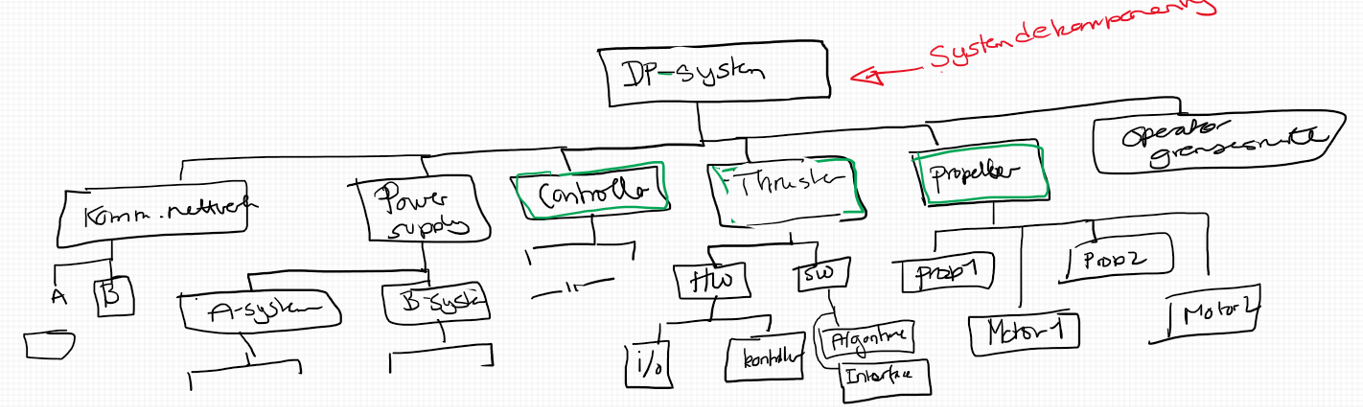
\includegraphics[width=\textwidth]{figures/FMECA/fmeca.PNG}\\
        \caption{Eksempel på systemdekomponering av et DP-system.}
        \label{fig:decomp}
\end{figure}

\begin{figure}[H]
    \centering
        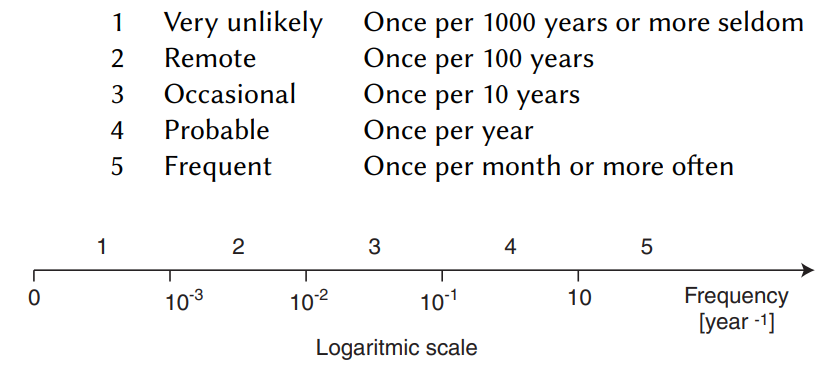
\includegraphics[width=\textwidth]{figures/FMECA/freq.PNG}\\
        \caption{Eksempel på klasser for feilrater.}
        \label{fig:feilrate}
\end{figure}

\begin{figure}[H]
    \centering
        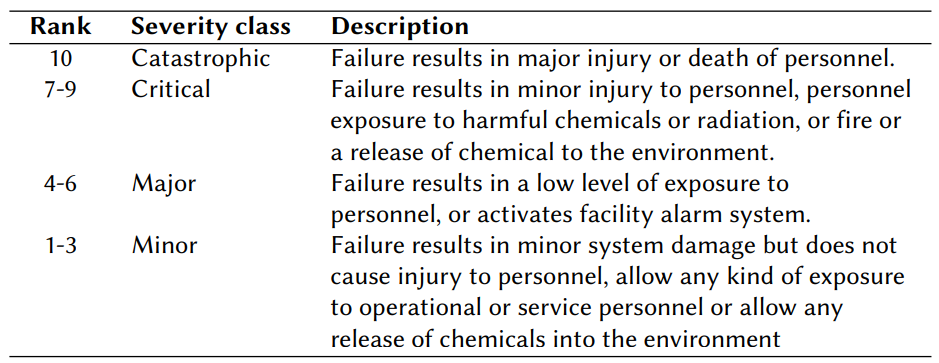
\includegraphics[width=\textwidth]{figures/FMECA/sever.PNG}\\
        \caption{Eksempel på klasser for alvorlighet.}
        \label{fig:alvor}
\end{figure}


\begin{figure}[H]
    \centering
        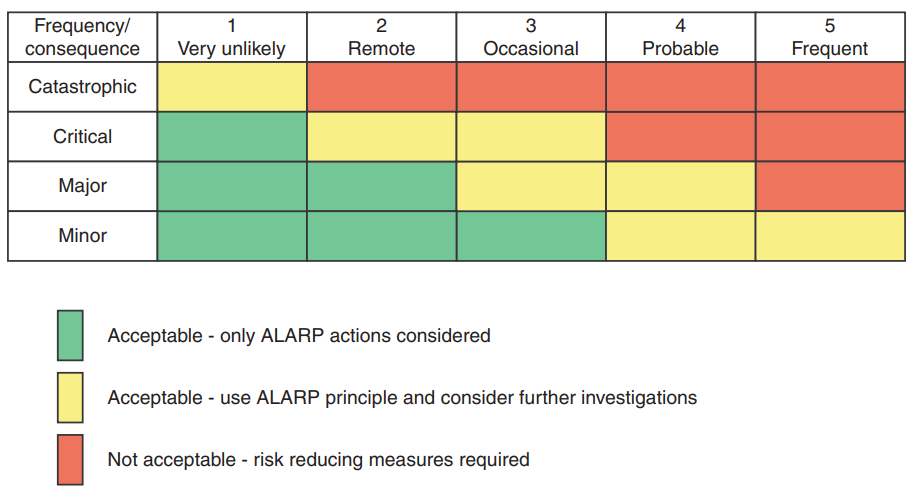
\includegraphics[width=\textwidth]{figures/FMECA/riskmat.PNG}\\
        \caption{Eksempel på risikomatrise brukt i FMECA.}
        \label{fig:riskmat}
\end{figure}

\subsection{Fordeler og ulemper med FMECA}

\textbf{Fordeler}

\begin{itemize}
    \item FMECA er en veldig strukturert og pålitelig metode for å evalurere systemer
    \item Konseptet er enkelt å lære, også for nybegynnere
    \item Tilnærmingen fjør at det er enkelt å analysere også ganske komplekse systemer.
\end{itemize}

\textbf{Ulemper}

\begin{itemize}
    \item FMECA-prosessen kan være kjedelig, tidkrevende og dermed også dyr
    \item Konseptet evaluerer ikke muligheten for flere feil på en gang, noe som ofte er
    tilfellet i praksis.
    \item Det er lett å neglisjere menneskelige feil i analysen.
\end{itemize}